% creator: ilyakooo0
% extra credit: dashared
% version: 1.0.1

\PassOptionsToPackage{main=russian,english}{babel}

\documentclass{../TechDoc}

\title{3D Xоррор-игра от первого лица на Unreal Engine 5 для ПК}
\author{Студент группы БПИ212}{М. С. Смагин}
\academicTeacher{Приглашенный преподаватель департамента программной инженерии факультета компьютерных наук}{Д. П. Архаров}

\documentTitle{Техническое задание}
\documentCode{RU.17701729.07.05-03 ТЗ 01-1}


\AtBeginDocument{\renewcommand\contentsname{\hfillСОДЕРЖАНИЕ\hfill}}
\begin{document}
    \maketitle
    
    \tableofcontents

    \addcontentsline{toc}{section}{СОДЕРЖАНИЕ}

    \section*{АННОТАЦИЯ}

Техническое задание – это основной документ, оговаривающий набор требований и
порядок создания программного продукта, в соответствии с которым производится разработка программы, ее тестирование и приемка.

Настоящее Техническое задание на разработку ``3D Xоррор-игра от первого лица на Unreal Engine 5 для ПК'' содержит следующие разделы: «Введение», «Основание для разработки», «Назначение разработки», «Требования к программе», «Требования к программным документам», «Технико-экономические показатели», «Стадии и этапы разработки», «Порядок контроля и приемки».

В разделе «Введение» указано наименование и краткая характеристика области применения ``3D Xоррор-игра от первого лица на Unreal Engine 5 для ПК''

В разделе «Основания для разработки» указан документ, на основании которого ведется разработка, и наименование темы разработки.

В разделе «Назначение разработки» указано функциональное и эксплуатационное
назначение программного продукта.

Раздел «Требования к программе» содержит основные требования к функциональным характеристикам, к надежности, к условиям эксплуатации, к составу и параметрам технических средств, к информационной и программной совместимости.

Раздел «Требования к программным документам» содержит предварительный состав программной документации и специальные требования к ней.

Раздел «Технико-экономические показатели» содержит ориентировочную экономическую эффективность, предполагаемую годовую потребность, экономические преимущества разработки 

Раздел «Стадии и этапы разработки» содержит стадии разработки, этапы и содержание работ.

В разделе «Порядок контроля и приемки» указаны общие требования к приемке работы.

Настоящий документ разработан в соответствии с требованиями:
\begin{enumerate}
    \item ГОСТ 19.101-77 Виды программ и программных документов [1]
    \item ГОСТ 19.102-77 Стадии разработки [2]
    \item ГОСТ 19.103-77 Обозначения программ и программных документов [3]
    \item ГОСТ 19.104-78 Основные надписи [4]
    \item ГОСТ 19.105-78 Общие требования к программным документам [5]
    \item ГОСТ 19.106-78 Требования к программным документам, выполненным печатным способом [6]
    \item ГОСТ 19.201-78 Техническое задание. Требования к содержанию и оформлению [7]
\end{enumerate}

Изменения к данному Техническому заданию оформляются согласно ГОСТ 19.603-78 [12], ГОСТ 19.604-78 [13].


    \clearpage

    \section{ВВЕДЕНИЕ}

\subsection{Наименование программы}

Наименование программы на русском языке: <<3D Xоррор-игра от первого лица на Unreal Engine 5 для ПК>>.

Наименование программы на английском языке: <<3D First-person Horror Game on Unreal Engine 5 for PC>>.

\subsection{Краткая характеристика области применения}

Программа является компьютерной видеоигрой, которая предлагает пользователям окунуться в мрачную игровую локацию заброшенного дома.  
Игроку предстоит выбраться из жуткого дома посредством решения различных головоломок, прячась от внутриигрового противника - похитителя.
Целевая аудитория программы - это любители хоррор-жанра и атмосферных игр с ограничением по возрасту: 18 лет.


    \clearpage

    \section{ОСНОВАНИЯ ДЛЯ РАЗРАБОТКИ}

\subsection{Документ, на основании которого ведётся разработка}

Учебный план подготовки бакалавров по направлению 09.03.04 «Программная инженерия» и утвержденная академическим руководителем программы тема курсового проекта.

    \clearpage
    
    \section{НАЗНАЧЕНИЕ РАЗРАБОТКИ}

\subsection{Функциональное назначение}

Функциональным назначением приложения является обеспечение возможности анализа HTML-документа любой сложности и извлечения из него любых представляющих интерес элементов. Программа должна уметь корректно обрабатывать страницы, контент на которых генерируется или модифицируется с помощью JavaScript, обеспечивая возможность извлечения динамически генерируемых элементов.

\subsection{Эксплуатационное назначение}

Приложение разрабатывается как компонент аналитической платформы данных ТОТ для <<СберАналитики>>.


    \clearpage

    \section{ТРЕБОВАНИЯ К ПРОГРАММЕ}

\subsection{Требования к функциональным характеристикам}

\subsubsection{Требования к составу выполняемых функций}

\begin{enumerate}
    % Сюжет - пока опускаем. В планах сделать "интро", в которой чел приезжает к дому, его учат управлению - это сюжет.
    % Меню
    \item[4.1.1.1.] Программа должна предоставлять возможность пользоватлелю загружать новую игровую\\
    сессию через стартовое меню;
    \item[4.1.1.2.] Программа должна предоставлять возможность пользователю посмотреть справку об игре\\
    из стартового меню;
    \item[4.1.1.3.] Программа должна предоставлять возможность выхода из игры через стартовое меню;
    \item[4.1.1.4.] Программа должна предоставлять возможность изменять громкость игры в меню \\настроек;
    \item[4.1.1.5.] Программа должна реализовывать возможность изменять экранный режим в меню \\настроек;
    \item[4.1.1.6.] Программа должна реализовать возможность изменять качество текстур в меню \\ настроек;
    \item[4.1.1.7.] Программа должна реализовать возможность выбирать сложность текущей игровой\\ 
    сессии в меню настроек;
    \item[4.1.1.8.] Программа должна предоставлять возможность менять яркость игрового освещения\\
    через меню настроек;
    \item[4.1.1.9.] Программа должна предоставлять возможность менять по отдельности\\
    громкость игрового окружения и громкость ИИ маньяка через меню настроек;
    % Меню ИИ
    \item[4.1.1.10.] Программа должна предоставлять пользователю возможность взаимодействовать с \\
    игровым миром через ИИ маньяка;
    \item[4.1.1.11.] Программа должна предоставлять пользователю возможность атаковать ИИ маньяка\\
    для использования эффекта изменения скорости перемещения маньяка \\по игровой локации;
    \item[4.1.1.12.] Программа должна реализовавывать атаку ИИ маньяка с потерей\\
    очков здоровья пользователя;
    \item[4.1.1.13.] Программа должна реализовывыть атаку ИИ маньяка с потерей\\ 
    очков выносливости пользователя;
    \item[4.1.1.14.] Программа должна реализовывать возможность перемещения\\
    ИИ маньяка ("шаг");
    \item[4.1.1.15.] Программа должна реализовывать возможность быстрого перемещения\\
    ИИ маньяка ("бег");
    \item[4.1.1.16.] Программа должна реализовывать возможность расставлять ловушки\\
    по игровой локации через ИИ маньяка;
    \item[4.1.1.17.] Программа должна реализовывать захвата камеры пользователя\\
    при использовании способности ИИ маньяка "похищение";
    \item[4.1.1.18.] Программа должна реализовывать анимацию ИИ маньяка;
    \item[4.1.1.19.] Программа должна реализовывать отображение информации\\
    о приближении ИИ маньяка к пользователю;
    % Карта: ловушки
    \item[4.1.1.20.] Программа должна реализовывать в окружении пользователя объекты\\
    ловушки, способные нанести урон игровому персонажу;
    \item[4.1.1.21.] Программа должна предоставвлять возможность обезвреживать ловушки\\
    по истечении времени с начала обезвреживания;
    \item[4.1.1.22.] Программа должна реализовывать анимацию атаки ловушки;
    \item[4.1.1.23.] Программа должна реализовывать анимацию обезвреживания ловушки;
    % Карта: Дом
    \item[4.1.1.24.] Программа должна реализовать локацию "Дом маньяка" с\\
    c возможностью перемещения игровых персонажей;
    \item[4.1.1.25.] Программа должна реализовывать анимацию внутреннего интерьера\\
    локации "Дом маньяка";
\end{enumerate}

\subsubsection{Организация входных данных}

Программа реагирует на ввод пользователя, который осуществляется через нажатия клавиш клавиатуры, левой кнопки мыши, передвижения мыши.
Эти входные данные включают в себя нажатия на кнопки мыши в процессе выбора опций в любых виджетах и меню.

\subsubsection{Организация выходных данных}

Программа визуализирует игровой процесс с использованием графических изображений. Она реагирует на изменения в отображении игрового мира в окне просмотра при перемещении игрового персонажа и вращении камеры. Кроме того, программа отображает различные виджеты и меню по командам, активируемым нажатием клавиш клавиатуры или левой кнопки мыши.


\subsection{Требования к надёжности}

\subsubsection{Обеспечение устойчивого функционирования}

\begin{enumerate}
    \item[4.2.1.1.] {Программа не должна аварийно завершаться при любых взаимодействиях пользователя с программой при соблюдении условий эксплуатаций (см. пункт 4.4).}
\end{enumerate}

\subsubsection{Контроль входной информации}

% Входные данные - клава и мышь, какой тут контроль писать??
Требования к контролю входной информации не предъявляются.

\subsubsection{Контроль выходной информации}

Требования к контролю выходной информации не предъявляются.

\subsubsection{Время восстановления после отказа}

\begin{enumerate}
    \item[4.2.2.1.] {Время восстановления после отказа работы программы не должно превышать 60 секунд.} 
\end{enumerate}

\subsection{Условия эксплуатации}

\subsubsection{Климатические условия эксплуатации}

Климатические условия эксплуатации совпадают с климатическими условиями эксплуатации, предъявляемыми к техническим устройствам, на которых запущена программа.

\subsubsection{Виды обслуживания}

Обслуживание не требуется. 

\subsubsection{Требования к численности и квалификации персонала}

Для управления системой достаточно одного человека, способного запустить на сервере систему управления базами.

\subsection{Требования к составу и параметрам технических средств}

Программа должна храниться и выполняться на устройстве, обладающим следующими минимальными техническими характеристиками:

\begin{enumerate}
    \item Свободный доступ в сеть Интернет
    \item Оперативная память: 1 ГБ
    \item Свободное место в постоянном хранилище данных: 10 ГБ
\end{enumerate}

\subsection{Требования к информационной и программной совместимости}

На устройстве должна быть установлена ОС Ubuntu версии 22.04 или выше. Устройство должно поддерживать браузер Google Chrome версии 75 или выше или браузер Mozilla Firefox версии 78 или выше, а также СУБД PostgreSQL версии 14.0 или выше и язык программирования Python версии 3.12 или выше.

\subsection{Требования к маркировке и упаковке}

Требования к маркировке и упаковке не предъявляются.

\subsection{Требования к транспортировке и хранению}

Исходный код должен храниться во внутреннем репозитории компании <<СберАналитика>>.

\subsection{Специальные требования}

Специальные требования не предъявляются.

    \clearpage

    \section{ТРЕБОВАНИЯ К ПРОГРАММНОЙ ДОКУМЕНТАЦИИ}

\subsection{Состав программной документации}

В состав программной документации должны входить следующие компоненты:
\begin{enumerate}
    \item "3D Xоррор-игра от первого лица на Unreal Engine 5 для ПК". Техническое задание (ГОСТ 19.201-78) [7]
    \item "3D Xоррор-игра от первого лица на Unreal Engine 5 для ПК". Пояснительная записка (ГОСТ 19.404-79) [10]
    \item "3D Xоррор-игра от первого лица на Unreal Engine 5 для ПК". Руководство оператора (ГОСТ 19.505-79) [11];
    \item "3D Xоррор-игра от первого лица на Unreal Engine 5 для ПК". Текст программы (ГОСТ 19.401-78) [9];
    \item "3D Xоррор-игра от первого лица на Unreal Engine 5 для ПК". Программа и методика испытаний (ГОСТ 19.301-79) [8];
\end{enumerate}


\subsection{Специальные требования к программной документации}

Документы к программе должны быть выполнены в соответствии с ГОСТ 19.106-78 [6] и ГОСТами к каждому виду документа (см. п. 5.1.).
Пояснительная записка должна быть загружена в систему Антиплагиат через SmartLMS <<НИУ ВШЭ>>.
Техническое задание и пояснительная записка, титульные листы других документов должны быть подписаны руководителем разработки и исполнителем. Документация и программа сдается в электронном виде в формате pdf или docx в архиве формата zip или rar.

За три дня до защиты комиссии все материалы курсового проекта:
\begin{enumerate}
    \item программная документация
    \item программный проект
    \item исполняемый файл
    \item отзыв руководителя
    \item отчет системы Антиплагиат
\end{enumerate}
должны быть загружены одним или несколькими архивами в проект дисциплины <<Курсовой проект>> в личном кабинете в информационной образовательной среде SmartLMS <<НИУ ВШЭ>>.


    \clearpage

    \section{ТЕХНИКО-ЭКОНОМИЧЕСКИЕ ПОКАЗАТЕЛИ}

\subsection{Ориентировочная экономическая эффективность}

В рамках данной работы расчёт экономической эффективности не предусмотрен.

\subsection{Предполагаемая потребность}

В видеоигровой индустрии существует постоянный спрос на новые хоррор-игры, как от известных международных компаний, так и от небольших объединений инди-разработчиков. Данный проект стремится создать жуткую внутриигровую локацию с множеством интерактивных предметов и компьютерным противником, чтобы предоставить страшное и интересное приключение игроку.

\subsection{Экономические преимущества разработки по сравнению с лучшими отечественными и зарубежными образцами или аналогами}

<<Универсальный парсер>> представляет собой индивидуальное решение, разработанное для предприятия <<СберАналитики>>, ключевые запрошенные заказчиком особенности:

\begin{itemize}
    \item настраиваемый кроулинг -- возможность переходить на ссылкам, найденным на изначально поданной странице
    \item упрощённая интеграция с остальными компонентами аналитической платформы
    \item независимость от первоначальной разметки страницы (универсальность)
    \item независимость от типа страницы (статичный HTML/динамичный SPA)
\end{itemize}

    \clearpage

    \section{СТАДИИ И ЭТАПЫ РАЗРАБОТКИ}

% Тем кто хочет это отредачить соболезную
\begin{tabular}{|l|l|l|l|}
  \hline
  \makecell[lt]{Стадия\\разработки} & \makecell[lt]{Этапы\\разработки} & \makecell[lt]{Содержание работ} & \makecell[lt]{Сроки\\выполнения} \\
  \hline
  \multirow[t]{2}{*}{\makecell[lt]{Техническое\\задание}} & \makecell[lt]{Обоснование\\необходимости\\разработки} & \makecell[lt]{Постановка задачи} & \makecell[lt]{01.01.2024-\\07.01.2024} \\
  \cline{2-4} 
  & \multirow{3}{*}{\makecell[lt]{Разработка и \\утверждение\\технического\\задания}} & \makecell[lt]{Определение требований к\\программе} & \makecell[lt]{15.01.2024-\\13.02.2024} \\
  \cline{3-4}
  & & \makecell[lt]{Определение стадий,\\этапов и сроков разработки\\программы и\\документации на нее} & \makecell[lt]{15.01.2024-\\13.02.2024} \\
  \cline{3-4}
  & & \makecell[lt]{Согласование и\\утверждение технического\\задания} & \makecell[lt]{13.02.2024-\\15.02.2024} \\
  \hline
  
  \multirow[t]{3}{*}{\makecell[lt]{Рабочий\\проект}} & \multirow[t]{3}{*}{\makecell[lt]{Разработка\\программы}} & \makecell[lt]{Разработка сюжета игры} & \makecell[lt]{16.01.2024-\\01.02.2024} \\
  \cline{3-4}
  & & \makecell[lt]{Разработка игровых локаций} & \makecell[lt]{01.02.2024-\\21.02.2024} \\
  \cline{3-4}
  & & \makecell[lt]{Разработка персонажа игрока\\и связанных механик} & \makecell[lt]{22.02.2024-\\18.03.2024} \\
  \cline{2-4}
  & \makecell[lt]{Разработка\\программной\\документации} & \makecell[lt]{Разработка программных\\документов} & \makecell[lt]{10.03.2024-\\14.03.2024} \\
  \cline{2-4}
  & \multirow[t]{3}{*}{\makecell[lt]{Испытания\\программы}} & \makecell[lt]{Разработка, согласование и\\утверждение порядка и\\методики испытаний} & \makecell[lt]{12.03.2024-\\14.03.2024} \\
  \cline{3-4}
  & & \makecell[lt]{Проведение\\предварительных\\испытаний} & \makecell[lt]{15.03.2024-\\20.03.2024} \\
  \cline{3-4}
  & & \makecell[lt]{Корректировка программы\\и программной\\документации по\\результатам испытаний} & \makecell[lt]{16.02.2024-\\23.03.2024} \\
  \hline
\end{tabular}

    \clearpage

    \section{ПОРЯДОК КОНТРОЛЯ И ПРИЁМКИ}

\subsection{Виды испытаний}
Производится проверка корректного выполнения программой заложенных в нее функций, то есть осуществляется функциональное тестирование программы. Функциональное тестирование осуществляется в соответствии с документом ``3D Xоррор-игра от первого лица на Unreal Engine 5 для ПК''. Программа и методика испытаний (ГОСТ 19.301-79) [8] в котором указывают:
\begin{enumerate}
    \item перечень функций программы, выделенных в программе для испытаний, и перечень требований, которым должны соответствовать эти функции (со ссылкой на пункт 4.1.1. настоящего технического задания)
    \item перечень необходимой документации и требования к ней (со ссылкой на пункты 5.1 и 5.2 настоящего технического задания)
    \item методы испытаний и обработки информации
    \item технические средства и порядок проведения испытаний; Сроки проведения испытаний обсуждаются дополнительно
\end{enumerate}

\subsection{Общие требования к приемке работы}

Прием программы будет утвержден при корректной работе программы в соответствии с пунктом 4.1.1 при различных входных данных, соответствующих условиям в пункте 4.1.2 данного документа и при предоставлении полной документации к продукту, указанной в пункте 5.1, выполненной в соответствии с требованиями, указанными в пункте 5.2 данного технического задания.

    \clearpage

    \section*{СПИСОК ИСПОЛЬЗОВАННЫХ ИСТОЧНИКОВ}
    \addcontentsline{toc}{section}{\protect\numberline{}СПИСОК ИСПОЛЬЗОВАННЫХ ИСТОЧНИКОВ}

    \begin{enumerate}
        \item ГОСТ 19.101-77 Виды программ и программных документов. //Единая система программной документации. – М.: ИПК Издательство стандартов, 2001. – 126 с
        \item ГОСТ 19.102-77 Стадии разработки. //Единая система программной документации. – М.: ИПК Издательство стандартов, 2001. – 126 с
        \item ГОСТ 19.103-77 Обозначения программ и программных документов. //Единая система программной документации. – М.: ИПК Издательство стандартов, 2001. – 126 с
        \item ГОСТ 19.104-78 Основные надписи. //Единая система программной документации. – М.: ИПК Издательство стандартов, 2001. – 126 с
        \item ГОСТ 19.105-78 Общие требования к программным документам. //Единая система программной документации. – М.: ИПК Издательство стандартов, 2001. – 126 с
        \item ГОСТ 19.106-78 Требования к программным документам, выполненным печатным способом. //Единая система программной документации. – М.: ИПК Издательство стандартов, 2001. – 126 с
        \item ГОСТ 19.201-78 Техническое задание. Требования к содержанию и оформлению. //Единая система программной документации. – М.: ИПК Издательство стандартов, 2001. – 126 с
        \item ГОСТ 19.301-79 Программа и методика испытаний. Требования к содержанию и оформлению. //Единая система программной документации. – М.: ИПК Издательство стандартов, 2001.
        \item ГОСТ 19.401-78 Текст программы. Требования к содержанию и оформлению. //Единая система программной документации. – М.: ИПК Издательство стандартов, 2001.
        \item ГОСТ 19.404-79 Пояснительная записка. Требования к содержанию и оформлению. //Единая система программной документации. – М.: ИПК Издательство стандартов, 2001.
        \item ГОСТ 19.505-79 Руководство оператора. Требования к содержанию и оформлению. //Единая система программной документации. – М.: ИПК Издательство стандартов, 2001
        \item ГОСТ 19.603-78 Общие правила внесения изменений. //Единая система программной документации. – М.: ИПК Издательство стандартов, 2001. – 126 с
        \item ГОСТ 19.604-78 Правила внесения изменений в программные документы, выполненные печатным способом. //Единая система программной документации. – М.: ИПК Издательство стандартов, 2001. – 126 с
    \end{enumerate}

    \clearpage

    \registrationList

    \raggedright\section*{\hfillПРИЛОЖЕНИЕ 1}
    \addcontentsline{toc}{section}{\protect\numberline{}ПРИЛОЖЕНИЕ 1}
    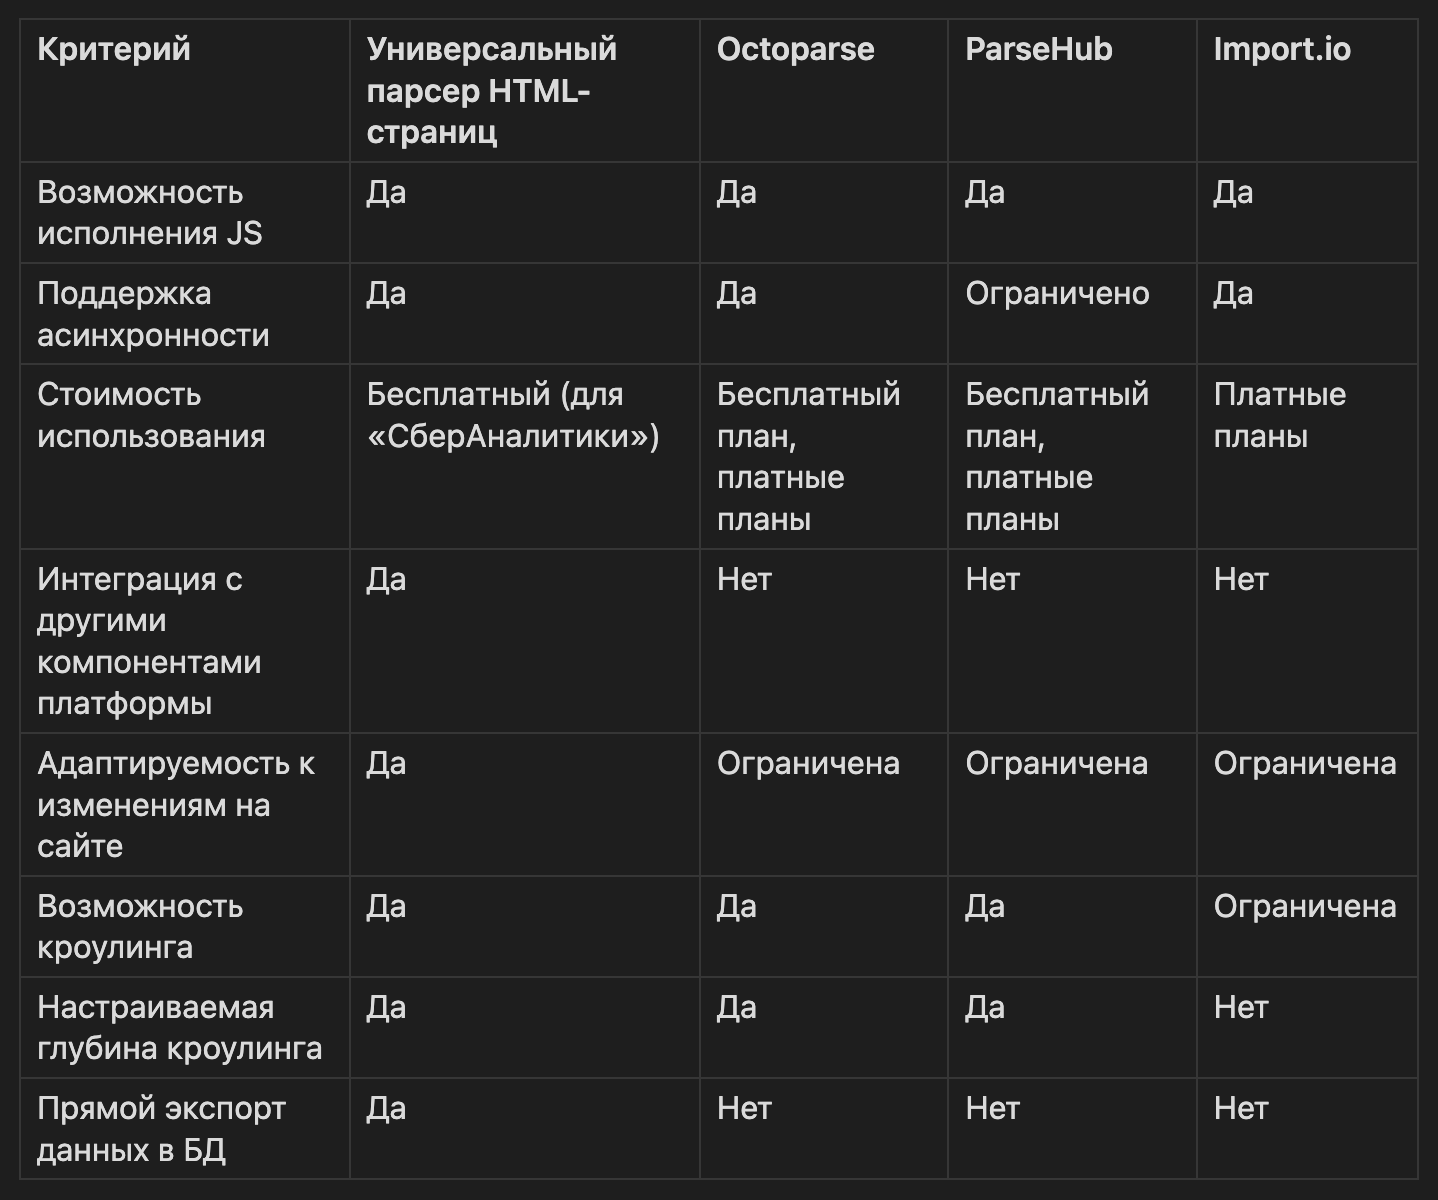
\includegraphics[width=\textwidth]{analogs}
        
\end{document}